\subsection{Descrizione dei canali al livello firmware}
\label{sct:ch_firmware}
Prima di descrivere l'implementazione delle forme di comunicazione considerate, viene descritto brevemente il protocollo tipico per realizzare la comunicazione di unit\`a di elaborazione firmware in modo indipendente dal tempo \cite{vanneschi2009architettura}. Le idee alla base di questo protocollo sono utilizzate per realizzare dei meccanismi efficienti e ottimizzati sull'architettura di \tile.
\begin{figure}[!b]
  \begin{subfigure}[b]{.5\textwidth}
    \centering
    \resizebox{.8\columnwidth}{!}{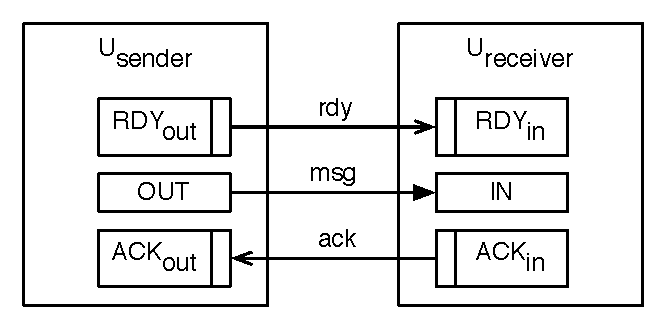
\includegraphics{firmware_communication.pdf}}
    \caption{Comunicazione simmetrica}
    \label{fig:fwcomm_sym}
  \end{subfigure}
  \begin{subfigure}[b]{.5\textwidth}
    \centering
    \resizebox{.8\columnwidth}{!}{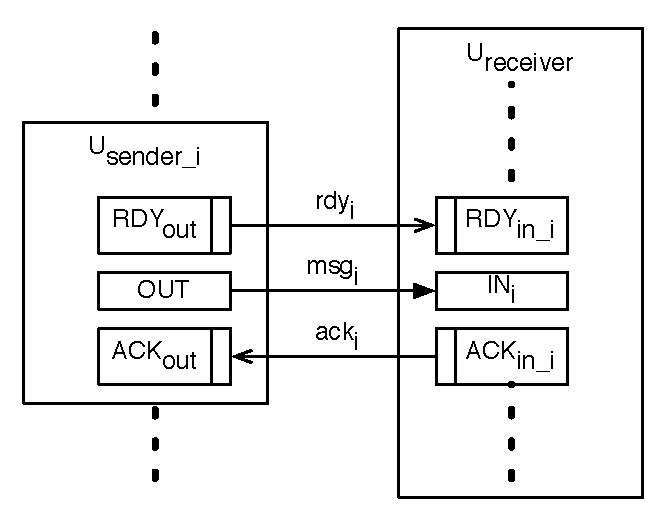
\includegraphics{firmware_asym_comm.pdf}}
    \caption{Comunicazione asimmetrica}
    \label{fig:fwcomm_asym}
  \end{subfigure}
  \caption{Componenti di un canale di comunicazione firmware}
  \label{fig:fwcomm}
\end{figure}

Si consideri la comunicazione simmetrica, il protocollo definisce due eventi: ``la presenza di un messaggio nel canale'' e ``la ricezione del messaggio da parte del ricevente''; nel livello firmware tali eventi sono realizzati tramite due collegamenti di un bit detti di Ready (Rdy) e di Acknowledgement (Ack) e da una coppia di indicatori di interfaccia per ciascun collegamento. Un canale di comunicazione a livello firmware \`e perci\`o costituito da tre componenti: l'interfaccia di uscita, il collegamento fisico e l'interfaccia di ingresso. Le interfacce contengono l'indicatore di uscita, quello di ingresso e il registro di uscita contenente il dato da trasmettere. Il collegamento \`e costituito dalle linee per connettere gli indicatori e i registri delle due interfacce. Un indicatore di interfaccia di uscita mette a disposizione l'operazione \emph{set} che provoca l'assunzione del valore 1 nell'indicatore di interfaccia di ingresso ad esso collegato. Un indicatore di interfaccia di ingresso mette a disposizione l'operazione \emph{test} con la quale viene letto il valore dell'indicatore, e l'operazione \emph{reset} con l'esecuzione della quale viene impostato a 0 il valore di uscita dell'indicatore stesso. Considerando due unit\`a $\mathrm{U}_{\mathrm{sender}}$ e $\mathrm{U}_{\mathrm{receiver}}$ collegate dai collegamenti \emph{rdy(1)}, \emph{msg(L)}, \emph{ack(1)} come in figura \ref{fig:fwcomm_sym}, il protocollo di comunicazione \`e perci\`o definito come in codice~\ref{lst:sym_firmware}
\begin{lstlisting}[language={}, morekeywords={msg, vtg}, float=t, caption={Descrizione astratta del protocollo di comunicazione del canale firmware simmetrico}, label={lst:sym_firmware}]
$\mathtt{U}_{\mathtt{sender}}$:send ::
  wait until $\mathtt{ACK}_{\mathtt{out}}$.test() is equal to 1
  send message msg to receiver and
    do $\mathtt{RDY}_{\mathtt{out}}$.set() and 
    do $\mathtt{ACK}_{\mathtt{out}}$.reset()

$\mathtt{U}_{\mathtt{receiver}}$:receive ::
  wait until $\mathtt{ACK}_{\mathtt{in}}$.test() is equal to 1
  use msg received and 
    do $\mathtt{ACK}_{\mathtt{in}}$.set() and
    do $\mathtt{RDY}_{\mathtt{in}}$.reset()
\end{lstlisting}

Il protocollo di comunicazione del canale asimmetrico in ingresso segue da quello descritto nel caso simmetrico: dal punto di vista logico \`e come se venissero adottati tanti canali simmetrici quante sono le unit\`a mittenti, ogni canale collega una unit\`a mittente all'unit\`a destinataria, figura \ref{fig:fwcomm_asym}. Il comportamento della funzione di invio rimane invariato rispetto a quello descritto precedentemente. Quello della funzione di ricezione testa tutti gli indicatori di tipo Rdy e con una certa politica ne seleziona uno tra quelli attivi ed esegue il protocollo del caso simmetrico, leggendo il valore, resettando il Rdy e inviando l'ack per il canale scelto.

